% 如果需要更新, 請email至: wufish@gmail.com
% 也可以到github留言: https://github.com/coldwufish/NYCU-thesis-template

% 載入會用到的套件, 通常不需要修改這邊的資料
\input{covers/load_env.tex} 

% 為了看起來比較協調, 目錄的語言改為全部英文 or 全部中文, 中英混雜有點奇怪.
% 要使用中文目錄可把下面的註解拿掉, 當\toggletrue{toc-use-cn}啟用才會使用中文目錄, 預設使用英文目錄
%\toggletrue{toc-use-cn}



% --------------------------------------------
% 在這邊寫自己的資料
\newcommand{\chineseTitle}{中文論文名字}
\newcommand{\englishTitle}{English Title}
\newcommand{\studentCnName}{學生名字}
\newcommand{\studentEnName}{XXXX Wu} % 書名頁
\newcommand{\studentEnNameA}{Wu, XXXX} % 封面用
% 英文名字有兩種寫法, 一個是姓在後, 一個是放前面. 

\newcommand{\advisorCnName}{指導教授}
\newcommand{\advisorEnName}{OOOO Tseng} % 書名頁
\newcommand{\advisorEnNameA}{Tseng, OOOO} % 封面用
\newcommand{\ThesisDate}{August 2022} % 碩論的日期
\newcommand{\ThesisDateTW}{中華民國~ 一一一年八月}
% --------------------------------------------


\begin{document}
\begin{CJK*}{UTF8}{bkai}


% =============================================================
% 封面的設定, 像是日期之類的 settings for cover 
\newgeometry{top=3cm,bottom=3cm,left=3cm,right=3cm}

% 1. 第一頁的封面, 記得修改系所
\input{covers/front.tex}        % 碩士論文的封面
\input{covers/front_phd.tex}    % 博士論文版的封面 博士論文版的封面

% 2. 第二頁的書名頁, 記得修改系所, 日期
% 目前的浮水印剛好可以把校名&相關資訊包在裡面, 如果論文名稱太長的話, 換行之後的外觀就沒那麼漂亮XD 有需要的話可以自行調成inside裡面的字體大小. 
% 目前是\LARGE, 可以再小一點: \Large, 再小一點: \large
\input{covers/inside.tex}       % 碩士論文的書名頁
\input{covers/inside_phd.tex}   % 博士論文版的書名頁 博士論文版的書名頁

\restoregeometry
% =============================================================

% 書名頁起至最後一頁皆須加入浮水印
\AddToShipoutPicture{
    \put(-30,0){
        \parbox[b][\paperheight]{\paperwidth}{%
            \vfill
            \centering
            {\transparent{0.2}\includegraphics[scale=0.6]{covers/logo.png}}%
            \vfill
        }
    }
}

% =============================================================

% 口試結束後, 會有一些文件(3&5)需要口委們簽名
% 這邊的東西是最後上傳到圖書館要加入的東西
% (我當年畢業不需要4 XD)

% 3. 論文電子檔著作權授權書: auth.pdf
%\includepdf[pages={1},pagecommand={\thispagestyle{empty}}]{auth.pdf}

% 4. 博士論文指導教授推薦書(碩士論文免附): phd_recommend.pdf
%\includepdf[pages={1},pagecommand={\thispagestyle{empty}}]{phd_recommend.pdf}

% 5. 學位論文審定同意書(審定書): approval_ch.pdf
%\includepdf[pages={1},pagecommand={\thispagestyle{empty}}]{approval_ch.pdf}

% =============================================================
% 目錄設定

\frontmatter
\pagenumbering{roman}
{\fontfamily{ptm}\selectfont

\iftoggle{toc-use-cn}
{ % true section. 使用中文
\renewcommand{\contentsname}{目錄} % 使用中文目錄

% 下面這些是要在目錄上加入...的符號與頁碼
\titlecontents{chapter}[0em]{}{第\CJKnumber{\thecontentslabel}章 \hspace{0.5em}}{}{\titlerule*{.}\contentspage}[\addvspace{1em}]
\titlecontents{section}[1.5em]{\addvspace{-0.5em}}{\thecontentslabel \hspace{1em}}{}{\titlerule*{.}\contentspage}[\addvspace{0.5em}]
\titlecontents{subsection}[3em]{}{\thecontentslabel \hspace{1em}}{}{\titlerule*{.}\contentspage}[\addvspace{0.5em}]

% 6. 致謝 Acknowledgement
\addcontentsline{toc}{chapter}{誌\,\,\,\,\,謝} \input{Sections/Acknowledgement}\newpage

% 7 中文摘要 chinese abstract
\addcontentsline{toc}{chapter}{中文摘要} 
  \begin{center}
	\large
    \begin{singlespace}    
      \textbf{\chineseTitle{}} \\[0.5cm]
    \end{singlespace}
    
    \begin{singlespace}    

    	學生      :\studentCnName{}  \hspace{2.5cm}  指導教授  :\advisorCnName \hspace{0.1cm} 博士 \\
         [0.5cm]

    \end{singlespace}
    

    國立陽明交通大學網路工程研究所碩士班 \\[0.5cm]
    \textbf{摘~~~~~~~~要} \\[0.5cm]

  \end{center}
  \normalsize 
  %\hspace{0.75cm}
  中文摘要就從這邊開始寫.

  \vspace{1cm}

  % 中文摘要及關鍵詞 5-7 個 
  \textbf{關鍵字:}中文, 摘要, 關鍵詞, 5-7個, 不要多, 也不要少
 \newpage

% 8. 英文摘要
\addcontentsline{toc}{chapter}{英文摘要}  \begin{center}
  	\large
  	\begin{singlespace}
  		\textbf{\englishTitle{}} \\[0.5cm]
  	\end{singlespace}
  	
  	\begin{singlespace}

  			Student : \studentEnName{}  \hspace{1.0cm} Advisor  : Dr.\, \advisorEnName \\
  			[0.5cm]

  	\end{singlespace}
  	
  	\begin{singlespace}
  		Institute of Network Engineering\\
  		National Yang Ming Chiao Tung University\\[0.5cm]
  	\end{singlespace}
  	\textbf{Abstract} \\[0.5cm]
  	
  \end{center}
  \normalsize 
  
%  \hspace{0.25cm}
Write your abstract here. Through computer vision technologies, ...


\vspace{1cm}

% 5-7 Keywords (English) 
\textbf{Keywords: English, keywords, five to seven, computer vision, IoT.} 
  
 \newpage

% 9. 目錄 中文版
\addcontentsline{toc}{chapter}{目錄} \tableofcontents \newpage

% 10. 圖片目錄 中文版
\renewcommand{\figurename}{圖} % 把caption的Figure改成"圖"
\renewcommand{\listfigurename}{圖目錄}
\renewcommand{\numberline}[1]{圖~#1\hspace*{1em}}
\addcontentsline{toc}{chapter}{圖目錄\vspace{0em}} \listoffigures \newpage

% 11. 表格目錄 中文版, 有需要再打開
\renewcommand{\tablename}{表} % 把caption的Table改成"表"
\renewcommand{\listtablename}{表目錄}
\renewcommand{\numberline}[1]{表~#1\hspace*{1em}}
\addcontentsline{toc}{chapter}{表目錄\vspace{0em}} \listoftables \newpage

% 把Chapter改成 第X章
\titleformat{\chapter}{\normalfont\huge\bfseries}{第\zhnum{chapter}章、}{0em}{}
\titleformat{\section}{\normalfont\Large\bfseries}{\thesection}{1em}{}
\titleformat{\subsection}{\normalfont\large\bfseries}{\thesubsection}{1em}{}
} % true end. 中文目錄設定結束
% ==========================================
% ==========================================
{ % false section. 使用英文目錄
\renewcommand{\contentsname}{Contents} % 使用英文目錄


% 下面這些是要在目錄上加入...的符號與頁碼
\titlecontents{chapter}[0em]{}{\thecontentslabel \hspace{1em}}{}{\titlerule*{.}\contentspage}[\addvspace{1em}]
\titlecontents{section}[1.5em]{\addvspace{-0.5em}}{\thecontentslabel \hspace{1em}}{}{\titlerule*{.}\contentspage}[\addvspace{0.5em}]
\titlecontents{subsection}[3em]{}{\thecontentslabel \hspace{1em}}{}{\titlerule*{.}\contentspage}[\addvspace{0.5em}]

% 6. 致謝 Acknowledgement
\addcontentsline{toc}{chapter}{Acknowledgement} \input{Sections/Acknowledgement}\newpage

% 7 中文摘要 chinese abstract
\addcontentsline{toc}{chapter}{Chinese Abstract} 
  \begin{center}
	\large
    \begin{singlespace}    
      \textbf{\chineseTitle{}} \\[0.5cm]
    \end{singlespace}
    
    \begin{singlespace}    

    	學生      :\studentCnName{}  \hspace{2.5cm}  指導教授  :\advisorCnName \hspace{0.1cm} 博士 \\
         [0.5cm]

    \end{singlespace}
    

    國立陽明交通大學網路工程研究所碩士班 \\[0.5cm]
    \textbf{摘~~~~~~~~要} \\[0.5cm]

  \end{center}
  \normalsize 
  %\hspace{0.75cm}
  中文摘要就從這邊開始寫.

  \vspace{1cm}

  % 中文摘要及關鍵詞 5-7 個 
  \textbf{關鍵字:}中文, 摘要, 關鍵詞, 5-7個, 不要多, 也不要少
 \newpage

% 8. english abstract
\addcontentsline{toc}{chapter}{English Abstract}  \begin{center}
  	\large
  	\begin{singlespace}
  		\textbf{\englishTitle{}} \\[0.5cm]
  	\end{singlespace}
  	
  	\begin{singlespace}

  			Student : \studentEnName{}  \hspace{1.0cm} Advisor  : Dr.\, \advisorEnName \\
  			[0.5cm]

  	\end{singlespace}
  	
  	\begin{singlespace}
  		Institute of Network Engineering\\
  		National Yang Ming Chiao Tung University\\[0.5cm]
  	\end{singlespace}
  	\textbf{Abstract} \\[0.5cm]
  	
  \end{center}
  \normalsize 
  
%  \hspace{0.25cm}
Write your abstract here. Through computer vision technologies, ...


\vspace{1cm}

% 5-7 Keywords (English) 
\textbf{Keywords: English, keywords, five to seven, computer vision, IoT.} 
  
 \newpage

% 9. 目錄 English version
\addcontentsline{toc}{chapter}{Contents} \tableofcontents \newpage

% 10. 圖片目錄 English version
\renewcommand{\numberline}[1]{Figure~#1\hspace*{1em}}
\addcontentsline{toc}{chapter}{List of Figures} \listoffigures \newpage

% 11. 表格目錄 English version, 有需要再打開
\renewcommand{\numberline}[1]{Table~#1\hspace*{1em}}
\addcontentsline{toc}{chapter}{List of Tables} \listoftables \newpage

% 調整內文的chapter, section, subection的顯示方式, 改成靠左對齊+沒有換行
\titleformat{\chapter}{\normalfont\huge\bfseries}{Chapter \thechapter.}{1em}{}
\titleformat{\section}{\normalfont\Large\bfseries}{\thesection}{1em}{}
\titleformat{\subsection}{\normalfont\large\bfseries}{\thesubsection}{1em}{}
} % false end. 使用英文


\mainmatter
\pagenumbering{arabic} % enabling page numbering


% =========================================================================
% 12. 論文正文, 可以每個章節一個.tex檔案 (put your statements in the following)

\chapter{Introduction}
\label{ch:intro}
內文可以直接打中文, 也可以寫英文. 學校有買英文學術寫作引導工具Writefull, 軟體功能有: 
(1)依照論文章節用途,提供句型建議、用語比較、論文用字建議等,並依使用比例提供不同選擇。
(2)修正文法與標點符號的誤用。
(3)偵測及提醒是否需要加註引用文獻。
(4)可逐步修正或一鍵訂正,並可標記修訂。
(5)與Microsoft Word整合,在寫作過程中直接給予建議。(其實overleaf也可以用)

詳情可參考: https://www.lib.nycu.edu.tw/custom?menu=125\&cid=411

Video-based surveillance systems have been widely used in places such as plaza, office, factory, hotel, and conference hall for security purposes\cite{collins2000system},\cite{wang2013intelligent}. 

The rest of this paper is organized as follows. Chapter 2 reviews some related work. Chapter 3 introduces our system architecture. Chapter 4 explains the details of our pairing algorithm. Performance evaluation results are in Chapter 5. Conclusions are in Chapter 6.
 \newpage
\chapter{Related Work}
\label{ch:relatedwork}
通常第二段就是寫相關的參考文獻, 只有cite到的文章才會出現編號並且出現在最後面. 舉例來說, 如果在ref.bib裡放了10篇論文, 可是內文只有cite其中五篇, 編譯出來的結果就只會顯示這五篇. Ref有很多種風格寫法, 本篇論文是採用bibliographystyle\{IEEEtran\}, 
overleaf上有其他style語法, 可以參考: \\
https://www.overleaf.com/learn/latex/Bibtex\_bibliography\_styles

This is related work. The PID issue has been widely studied in the field of computer vision and IoT by using various devices. In the field of computer vision, camera is the most popular device. Face recognition technologies are surveyed in \cite{zhao2003face}. Reference \cite{parkhi2015deep} focuses on how to collect a very large training dataset and build a very deep CNN model for face recognition, but training process is extremely computationally expensive. A hybrid RFID and computer vision system for localization and tracking of RFID tags is proposed in \cite{goller2014fusing}. Reference \cite{isasi2010location} presents a solution which combines RFID with object tracking through cameras. Reference \cite{germa2010vision} presents a fusion system consisting of an RFID reader and a camera crew on a mobile robot platform to track people. These works \cite{goller2014fusing},\cite{isasi2010location},\cite{germa2010vision} fuse data from camera and RFID, but their accuracy highly depends on the density of RFID antennas. Thus, they are not suitable for longer range PID. Reference \cite{munaro2014fast} proposes a fast multi-people tracking algorithm for service robots through RGB-D camera. In \cite{spinello2011people}, people detection is realized by dense depth data, called Histogram of Oriented Depths (HOD).  \newpage
\chapter{System Model}
\label{ch:architecture}

如果想在latex裡面插入表格, 可以搜尋latex table generator, 有很多線上網站可以參考. 我個人都是使用線上網站去產生大致的語法, 然後再根據個人喜好去做微調, wikibook有很多資料可以參考, 網址在這邊: https://en.wikibooks.org/wiki/LaTeX/Tables

如果要引用表格, 記得在table裡加上label的語法, 然後就可以呼叫 Tab~\ref{tab1}, 寫中文的就是表~\ref{tab1}. 通常Table的caption是寫在表格的上面, 圖片則是放在下面.

\begin{table}[!ht]
    \centering
    \caption{This is a table.}
    \label{tab1}
    \begin{tabular}{|l|l|l|l|}
    \hline
        A & 1 & 4 & 7 \\ \hline
        B & 2 & 5 & 8 \\ \hline
        C & 3 & 6 & 9 \\ \hline
    \end{tabular}
\end{table}
 \newpage
\chapter{Data Fusion Algorithm}
\label{ch:method}

這個是插入圖片的範例, 圖片都放在img資料夾裡面. 檔案格式有支援: JPG, PNG, PDF, EPS. 就使用自己習慣的繪圖工具, 比較常見的應該就是power point!? power point可以把繪圖區另存成JPG, PNG, 還有SVG (新版才有, 我用的office 2016沒有這選項 QQ). SVG可以再轉成PDF, 這樣圖片縮放還是會很清楚, 可以把範例的兩張圖片都放大來看, 應該可以看出差別. 我個人都是用visio來畫圖, 可是都找不到替代工具, 如果有好用的繪圖工具麻煩分享交流一下 QQ 也看過蠻多人用draw.io, 只是這個用起來不太順手. orz
圖片出現的位置是由latex去決定, 有時候會出現在奇怪的地方, 這時候只能多爬文、嘗試各種參數, 或者把整段圖片code放在前面試試看.

overleaf上有插入圖片的介紹: https://www.overleaf.com/learn/latex/Inserting\_Images


    \begin{figure}
      \centering
      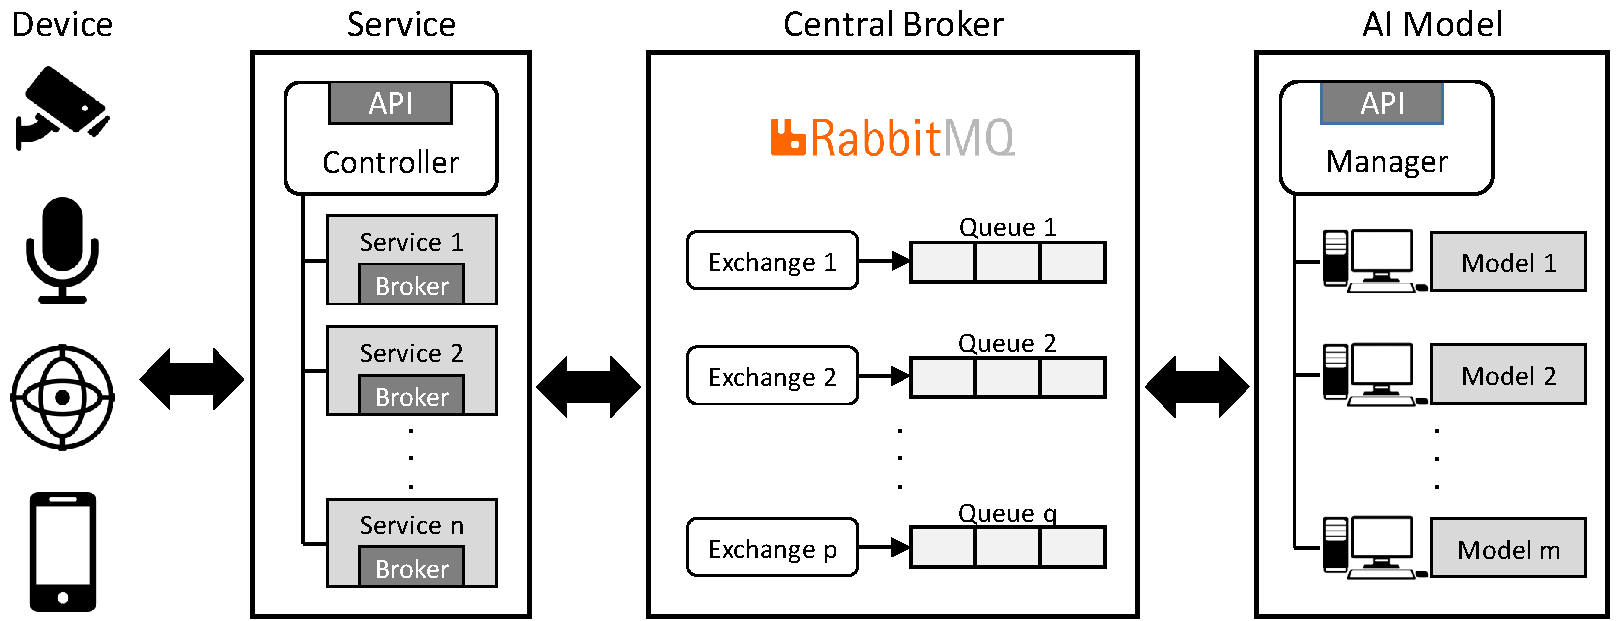
\includegraphics[width=1\columnwidth]{img/1.system_architecture.pdf}
      \caption{PDF圖檔範例.} 
      \vspace{-0.4cm}
      \label{fig:system_architecture}
    \end{figure}

\begin{figure}[htb]
	\centering
	\includegraphics[width=0.6\textwidth]{img/data_preprocessing.png}
	\caption{PNG example.}
	\label{fig:model}
\end{figure}

\section{Data Preprocessing}
\label{sec:SMA}
An example for section. Fig~\ref{fig:system_architecture} is PDF. Fig~\ref{fig:model} is PNG.


\subsection{2D LiDAR Data}
An example for subsection. 寫中文就是 圖~\ref{fig:system_architecture} 跟圖~\ref{fig:model}.
 \newpage
\chapter{Performance Evaluation}
\label{ch:evaluation}

In this section, 整理效能評估.
 \newpage
\chapter{Conclusions}
\label{ch:conclusion}
Write your conclusion here.
 
 \newpage
% =========================================================================


% =========================================================================
% 參考文獻的檔案 Reference file: ref.bib
% ref的寫法可以參考這邊: https://hackmd.io/Bc1-FIIISka6DW15sPprAw
\ClearShipoutPicture % 把ref的浮水印關掉

\iftoggle{toc-use-cn} % 使用中文
{\addcontentsline{toc}{chapter}{參考文獻}
\renewcommand{\bibname}{參考文獻} } 
{\addcontentsline{toc}{chapter}{References}
\renewcommand{\bibname}{References}
} 

\bibliographystyle{IEEEtran}
\bibliography{ref}
}
% =========================================================================


\end{CJK*}
\balance

\end{document}
